% !TeX root = POSTER.tex
\documentclass[25pt, a0paper,
portrait,
% landscape,
margin=2mm, 
innermargin=2mm, 
blockverticalspace=7mm, %distance between upper and lower block
colspace=2mm, %distance between left and right block 
subcolspace=0mm]{tikzposter}
		
% -- Packages --------------------------------------------------------%
\usepackage{amsfonts,amssymb,amsmath,mathtools}
\usepackage{defcmlfont}
\usepackage{tikz,lipsum}

\usepackage[T1]{fontenc}
% \usepackage{lmodern}
% \usepackage[english]{babel}

\usetikzlibrary{positioning}
\usepackage{float}                           % for minipages at Polarization part
\usepackage{caption}                         % no "Figure" in caption
\captionsetup[figure]{labelformat=empty}

\usepackage{psfrag}

% Load figures command: \inputfig [htb]{fig_dir}{fig_label}
\newcommand*{\inputfig}[3][htb]{{
    \def\fps@figure{#1}
    \def\DIR{#2}
    \def\LABEL{#3}
    \graphicspath{{\DIR/}}
    \psfrag{Al0}[c][c] {$\text{Al-doped LLZO}$}
\psfrag{Al2}[c][c] {$\text{Al-doped LLZO}$}
\psfrag{Tt0}[c][c] {$\text{Ta-doped LLZO}$}
\psfrag{Tt2}[c][c] {$\text{Ta-doped LLZO}$}
% \psfrag{ll}[c][c] {$\text{LLZO}$}
\psfrag{tem1}[c][c] {$\text{DFT($0^{\circ}K$)}$}
\psfrag{tem2}[c][c] {$\text{DFT($298^{\circ}K$)}$}

\psfrag{s1}[c][c] {\tiny $\text{a}_{\text{crevice}}\!=1\%$}
\psfrag{s2}[c][c] {\tiny $\text{a}_{\text{crevice}}\!=5\%$}
\psfrag{s3}[c][c] {\tiny $\text{a}_{\text{crevice}}\!=10\%$}
\psfrag{s4}[c][c] {\tiny $\text{a}_{\text{crevice}}\!=30\%$}
\psfrag{s5}[c][c] {\tiny $\text{a}_{\text{crevice}}\!=50\%$}

\psfrag{ca1}[c][c] {\footnotesize $10$}
\psfrag{ca2}[c][c] {\footnotesize $30$}
\psfrag{ca3}[c][c] {\footnotesize $1$}
\psfrag{ca4}[c][c] {\footnotesize $16$}
\psfrag{ca5}[c][c] {\footnotesize $50$}
\psfrag{ca6}[c][c] {\footnotesize $110$}

\psfrag{uca1}[c][c] {\footnotesize kPa}
\psfrag{uca2}[c][c] {\footnotesize kPa}
\psfrag{uca3}[c][c] {\footnotesize MPa}
\psfrag{uca4}[c][c] {\footnotesize MPa}
\psfrag{uca5}[c][c] {\footnotesize MPa}
\psfrag{uca6}[c][c] {\footnotesize MPa}

\psfrag{cr}[c][c] {$\text{crevice}$}
\psfrag{pp}[c][c] {$\text{Pre-existing crevice length}$}

\psfrag{a1}[c][c] {\tiny $1.000$}
\psfrag{b1}[c][c] {\tiny $0.950$}
\psfrag{c1}[c][c] {\tiny $0.911$}
\psfrag{d1}[c][c] {\tiny $0.866$}
\psfrag{e1}[c][c] {\tiny $0.866$}

\psfrag{a2}[c][c] {\tiny $1.000$}
\psfrag{b2}[c][c] {\tiny $0.950$}
\psfrag{c2}[c][c] {\tiny $0.904$}
\psfrag{d2}[c][c] {\tiny $0.859$}
\psfrag{e2}[c][c] {\tiny $0.866$}

\psfrag{a3}[c][c] {\tiny $1.00$}
\psfrag{b3}[c][c] {\tiny $0.950$}
\psfrag{c3}[c][c] {\tiny $0.985$}
\psfrag{d3}[c][c] {\tiny $0.936$}
\psfrag{e3}[c][c] {\tiny $0.866$}

\psfrag{a4}[c][c] {\tiny $0.899$}
\psfrag{b4}[c][c] {\tiny $0.854$}
\psfrag{c4}[c][c] {\tiny $1.000$}
\psfrag{d4}[c][c] {\tiny $0.950$}
\psfrag{e4}[c][c] {\tiny $0.866$}

\psfrag{a5}[c][c] {\tiny $0.948$}
\psfrag{b5}[c][c] {\tiny $0.900$}
\psfrag{c5}[c][c] {\tiny $1.000$}
\psfrag{d5}[c][c] {\tiny $0.950$}
\psfrag{e5}[c][c] {\tiny $0.866$}

\psfrag{a6}[c][c] {\tiny $0.956$}
\psfrag{b6}[c][c] {\tiny $0.908$}
\psfrag{c6}[c][c] {\tiny $1.000$}
\psfrag{d6}[c][c] {\tiny $0.950$}
\psfrag{e6}[c][c] {\tiny $0.866$}

\psfrag{ntn}[c][c] {\footnotesize \begin{tabular}{@{}c@{}} Stacking \\ Pressure \end{tabular}}

% \psfrag{tt1}[c][c] {\textsc{Griffith} criterion on
% ($\textbf{100}$-Li-termination)-$\{\textbf{50}\text{Ta}^{\bullet}_{\text{Zr}}\}$-doped-$\glssymbol{llzo}$ at T=298$^{\circ}$K}

% \psfrag{tt2}[c][c] {Percentage of pre-existing crevice per unit length at
% (\acrshort{li}$|$$\{\textbf{50}\text{Ta}^{\bullet}_{\text{Zr}}\}$-\acrshort{llzo})-Interface}

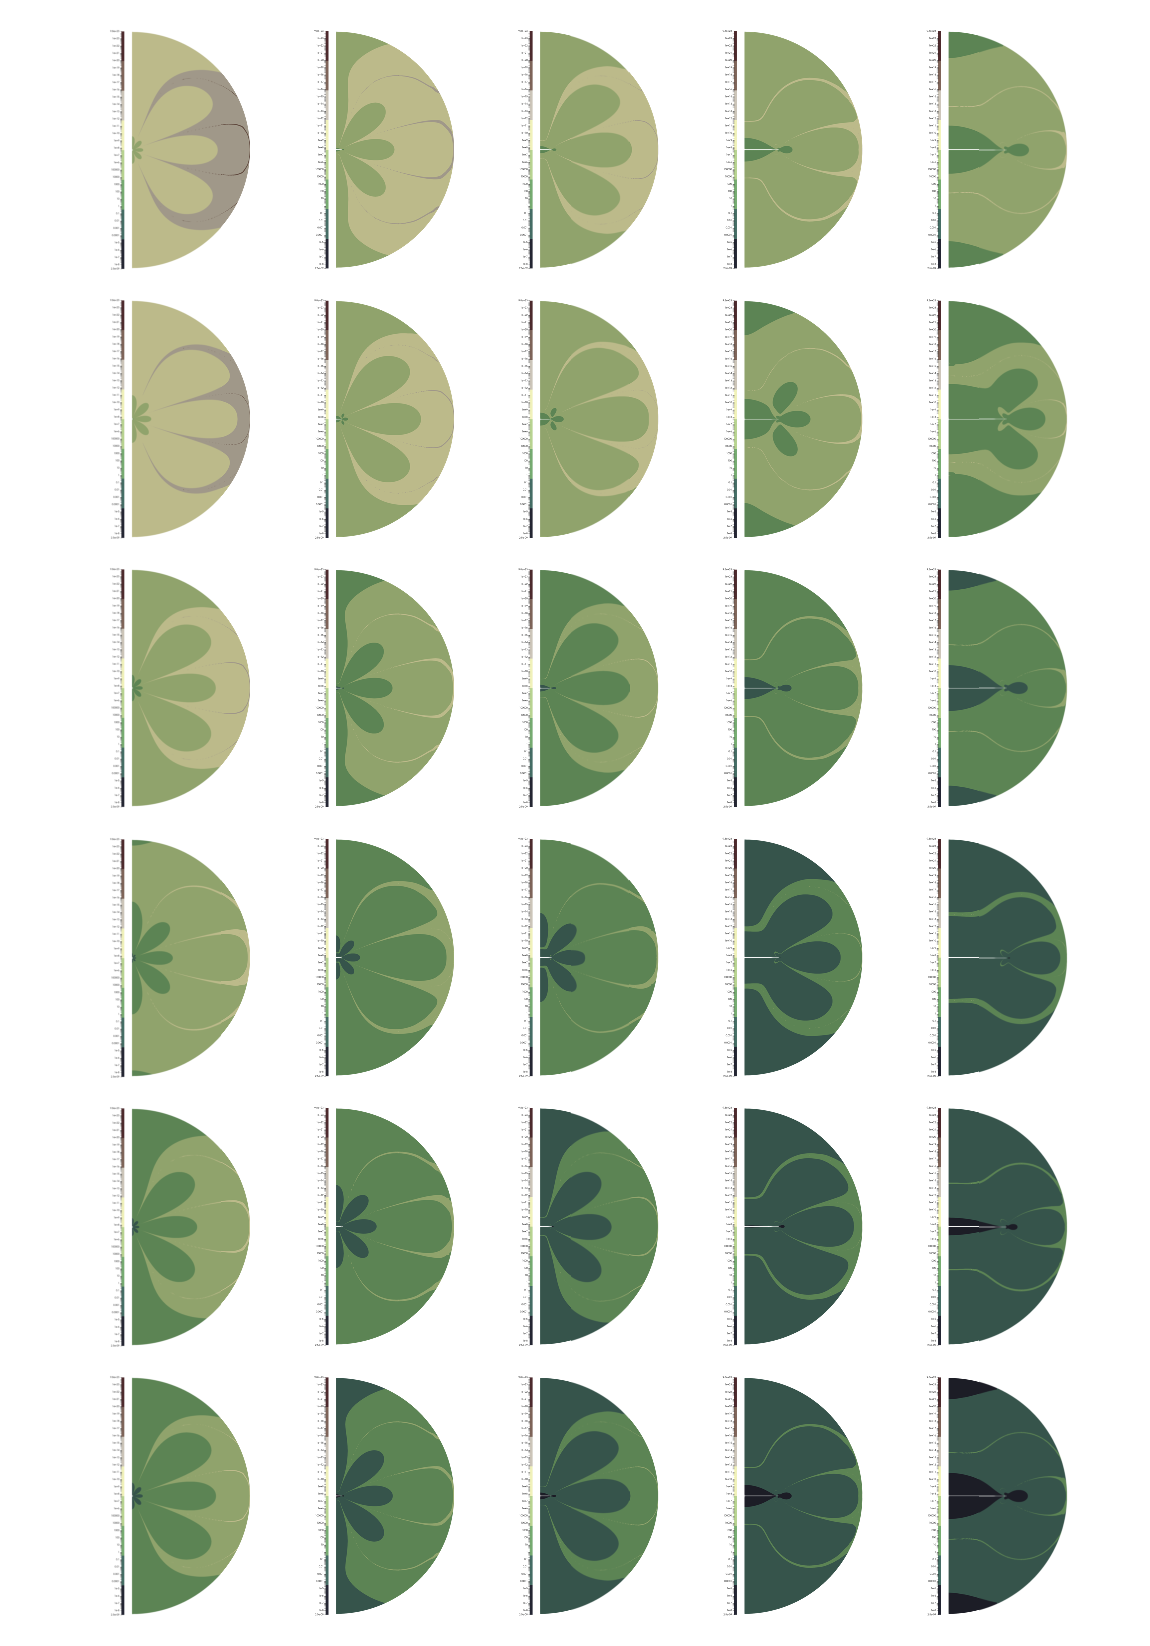
\includegraphics[width=0.6\textwidth]{contour_figs_Griffith_xx_Ta_pressure_crevice_298K.eps}
}}

\usepackage{fontawesome}
\usepackage{bm}
\usepackage{bigints}
\usepackage{relsize}

\usepackage{accents}

\usepackage{lipsum} 

\usepackage{babel}
\usepackage{hyperref}
\usepackage{cleveref}

\usepackage{mdframed}

\usepackage{xcolor}

% double int with circle \oiint
\usepackage{esint}

\usepackage{cancel}

% \usepackage[dvipsnames]{xcolor}

% -- Commands --------------------------------------------------------%
% \newcommand{\wall}{\text{w}}
% \newcommand{\interf}{\text{i}}
% \newcommand{\phase}{k}	
% \newcommand{\liquid}{\ell}
% \newcommand{\steam}{g}
% \newcommand{\out}{\text{out}}
% \newcommand{\tr}{{\mathsf T}}
\newcommand{\WA}{\prescript{\mathcal{W}}{}{\!\!\!\mathcal{A}}}
\newcommand{\WAz}{\prescript{\mathcal{W}}{}{\!\!\!\mathcal{A}}(z)}
\newcommand{\WApz}{\prescript{\mathcal{W}}{}{\!\!\!\mathcal{A}}'(z)}
\newcommand{\WAxx}{\prescript{\mathcal{W}}{}{\!\!\!\mathcal{A}}(x_1,x_2)}

\newcommand{\WAsigma}{\prescript{\prescript{\mathcal{W}}{}{\!\!\!\mathcal{A}}}{}{\!\sigma}}
\newcommand{\WABsigma}{\prescript{\prescript{\mathcal{W}}{}{\!\!\!\mathcal{A}}}{}{\!\boldsymbol{\sigma}}}

% Mathematic sets
\newcommand{\mbR}{\mathbb{R}}
\newcommand{\mbC}{\mathbb{C}}

% mathcals
\newcommand{\mcA}{\mathcal{A}}
\newcommand{\mcB}{\mathcal{B}}
\newcommand{\mcC}{\mathcal{C}}
\newcommand{\mcD}{\mathcal{D}}
\newcommand{\mcE}{\mathcal{E}}
\newcommand{\mcO}{\mathcal{O}}
\newcommand{\mcS}{\mathcal{S}}
\newcommand{\mcT}{\mathcal{T}}
\newcommand{\mcV}{\mathcal{V}}
\newcommand{\mcW}{\mathcal{W}}

\newcommand{\mcK}{\mathcal{K}}
\newcommand{\mcM}{\mathcal{M}}
\newcommand{\mcZ}{\mathcal{Z}}

\newcommand{\bigoiintsss}{\mathlarger{\mathlarger{\varoiint}}}
\newcommand{\bigoiintssss}{\mathlarger{\varoiint}}
\newcommand{\bigoiintsssss}{\varoiint}

\newcommand{\Kipc}{\mathcal{K}^{c}}
\newcommand{\Kipcz}{\mathcal{K}^{c}(z)}

% -- Title, Author, Institute --------------------------------------------------------%
% \title{
% \begin{minipage}{0.22\textwidth}
% 	
\includegraphics[width=1.02\textwidth]{./floats/logos/siam_siamcse23.eps}
% \end{minipage}
% \hfill
% \begin{minipage}{0.46\textwidth}
% 	\begin{flushleft}
% 		{\bfseries Next-generation all-solid-state battery}
% 	\end{flushleft}
% 	% \author{\underline{Tuan Vo}$^{\text{a,b}\,\dagger}$, Claas Hüter$^{\text{b}}$, Stefanie Braun$^{\text{a}}$, Manuel Torrilhon$^{\text{a}}$}
% 	% {\normalsize \underline{Tuan Vo}$^{\text{a,b}\,\dagger}$, Claas Hüter$^{\text{b}}$, Stefanie Braun$^{\text{a}}$, Manuel Torrilhon$^{\text{a}}$}
% \end{minipage}
% \hfill
% \begin{minipage}{0.22\textwidth}
% 	% \begin{flushleft}
% 		
\includegraphics[width=1.02\textwidth]{./floats/logos/rwth_acom_en_cmyk_fzj_gap.eps}
% 	% \end{flushleft}
% \end{minipage}
% }
% \title{\scshape Next-generation all-solid-state battery (\#ASSB @ \#OBMS23)}
% \title{\scshape Mathematical modelling for all-solid-state battery:\!\! (se|sse)-Interface}
\title{\scshape Mathematical modelling for All-solid-state battery}
\author{
	\underline{Tuan Vo}$^{\text{a,b}\,\dagger}$, Claas Hüter$^{\text{b}}$, Stefanie Braun$^{\text{a}}$, Manuel Torrilhon$^{\text{a}}$\\
\normalsize vo@acom.rwth-aachen.de}
\author{\underline{Tuan Vo}$^{\text{a,b}\,\dagger}$, Claas Hüter$^{\text{b}}$, Stefanie Braun$^{\text{a}}$}
\institute{\large
$\prescript{a}{}{}$Department of Mathematics, Applied and Computational Mathematics (ACoM), 
RWTH Aachen University, Schinkelstraße 02, 52062 Aachen, Germany\\
$\prescript{b}{}{}$Institute of Energy and Climate Research (IEK-2), 
Forschungszentrum Jülich, Wilhelm-Johnen-Straße, 52428 Jülich, Germany
}

% \titlegraphic{
\includegraphics[height=6cm]{./figs/FZJ_only.pdf} \hfill 
\includegraphics[height=6cm]{./figs/rwth_mathcces_bild_rgb_only.pdf} }
% \titlegraphic{
\includegraphics[width=0.3\textwidth]{./floats/logos/rwth_acom_en_cmyk_siamcse23_fzj_gap.eps}}

% \renewcommand{\familydefault}{\sfdefault} % Change font family

\bibliographystyle{plain}

\newcommand{\newcaption}[2]{\parbox{#1}{\centering{\small \it #2\par}}\normalsize}

% -- Predefined Colors and Themes ---------------------- %
% Choose THEME:  Default, Basic, Rays, Simple, Envelope, Wave, Board, Autumn, Desert,
% Explanation THEME: Default(gray+blueBC), Basic(green light), Rays(blue), 
% Simple(red), Envelope(Bluefancy), Wave(Bluefancy2), Board(Bluelight), Autumn(squarebox+bluebrown), Desert(squarebox+bluebrown2),
\usetheme{Default}

\useblockstyle[titleinnersep=0.7mm]{Default}    % change default parameter for title inner sep
% Choose COLOR STYLE:  Default, Blue, BlueGray, BlueOrange, BlueViolet, DarkBlue, GrayBlue, GrayLightblue, GrayRed, Green, GreenOrange, YellowRed
%\definecolor{main}{HTML}{0080FF}
%\definecolor{sub}{HTML}{8CDBFF}
%\usecolorstyle[colorOne=sub, colorTwo=main]{Default}

\definecolor{myoxford}{HTML}{002147}

\definecolor{blueoxford}{HTML}{002147}
\definecolor{redstanford}{HTML}{8C1515}

% ---------------------------------------------------------------------------------------------------------------- %
\begin{document}
% Title block
\maketitle[width=810mm]
% ---------------------------------------------------------------------------------------------------------------- %
\block{\bfseries Mathematical modelling for the next-generation All-solid-state batteries: Nucleation $\text{(SE|SSE)}^{\!(*)}$-Interface}
{
	\begin{minipage}{0.56\textwidth}
		\begin{minipage}{0.5\textwidth}
			\begin{mdframed}
				\textbf{Rechargeable Lithium-ion battery} (LIB)
				is at the heart of every electric vehicle (EV),
				portable electronic device,
				and energy storage system \cite{vo2018}.
				Nowadays, LIBs enable human life more efficient
				and help to solve global environment issues
				thanks to EVs' zero emission.
				However, conventional LIB (c-LIB)
				is sensible to temperature and pressure,
				hence, flammable and explosive, which is undesirable.
				% \colorbox{pink}{undesirable}.
				This bottleneck is
				mainly due to \textcolor{redstanford}{liquid-based electrolyte}
				found in c-LIBs.
			\end{mdframed}
		\end{minipage}
		%
		\begin{minipage}{0.49\textwidth}
			\begin{mdframed}
				\textbf{All-solid-state battery} (ASSB) is 
				one of promising candidates to overcome bottlenecks of c-LIBs. 
				Thanks to \textcolor{redstanford}{solid-state electrolyte} (SSE),
				ASSB is highly stable towards temperature and pressure. 
				Nevertheless, Li-metal dendrite 
				triggered at (SE|SSE)-Interface
				is the main drawback of ASSB
				since these dendritic threads
				extrapolate into SSE grain boundary network, 
				causing crevice, degradation of ionic conductivity,
				and the probability of short-circuit, which is 
				unfavorable \cite{hueter2017}.
				% \colorbox{pink}{unfavorable}.
			\end{mdframed}
		\end{minipage}
		%
		\begin{mdframed}
			\textbf{Next-generation All-solid-state battery} (ng-ASSB)
			with a consideration of \textcolor{redstanford}{nucleation criterion} defined by
			% \begin{align*}
			% 	a_{\text{Griffith}} := a^{*} = \arg\min_{a\in\mathbb{R}}{\bigintsss\!\!\!\!\!\!\bigintsss\!\!\!\!\!\!\bigintsss_{\Omega} f(a,\bm{u},\theta;\lambda,\mu,\bm{d}^{(\star)}\otimes\bm{d}^{(\star)}) \, d\Omega - \bigintsss\!\!\!\!\!\!\bigintsss_{\Gamma} f(a;\gamma) \, d\Gamma}\Bigg|_{\bar{\bm{u}}}
			% \end{align*}
			\begin{align}
				 & \rho_{\text{\tiny SCL}}\,
				\frac{D^2 \Bu_{\text{\tiny SCL}}}{D t^2}
				+
				\nabla \cdot
				\Big(
				% \accentset{\scriptstyle 4}{\mathbb{C}}^{f_{\text{alocation}}(\lambda,\mu,\Bd^{R}_{G_i, i=1,\dots,N},\Bd^{E};\Bx)}
				\mathbb{C}(\lambda,\mu)
				:\nabla\Bu^{(s)}_{\textsc{scl}}
				\Big)
				+ \rho_{\textsc{scl}}\,\Bb
				= -\rho_{\textsc{scl}}\,\nabla V_{e}, \\
				%--------------------------------
				\text{s.t.}\ \
				 & 
				a_{\text{Griffith}}^{\text{generalised}} := a^{*}
				= \arg \{ \min_{a\in\mathcal{V}}
				{
				\bigintsss\!\!\!\!\!\!\bigintsss\!\!\!\!\!\!\bigintsss_{\Omega}
				\!\!
				f(a_{\text{crevice}},\bm{u}_{\textsc{scl}},\theta_{\textsc{scl}},n^{\text{\tiny Li}^{\tiny +}};\lambda,\mu,\bm{d}_{\textsc{scl}}\otimes\bm{d}_{\textsc{scl}}) \, d\Omega
				- 
				\!\!\!\!
				\bigintsss\!\!\!\!\!\!\bigintsss_{\Gamma}
				\!\!
				f(a_{\text{crevice}};\gamma) \, d\Gamma
				}
				\},
			\end{align}
			hold for $\forall\,a\in\mathcal{V}$.
			Here, $V_{e}: \mathbb{R}^{3}\to\mathbb{R}$
			is the electric potential applied globally on ASSB.
			Due to nature setting of ASSB taking the form
			(SE|SSE|SE)
			the electric potential becomes uniform.
			Additionally,
			$\Bu$ is the displacement field,
			$\theta$ temperature field,
			$a$ crevice length,
			$\lambda, \mu$ Lam\'{e} constants,
			$\Bd\otimes\Bd$ embedded misorientation SCL structural tensor,
			and
			$\gamma$ cracking-surface energy density,
			% \colorbox{pink}{can help}
			can help
			to improve ASSB performance
			\cite{vo2023_obms23}\cite{vo2023_cse23}.
		\end{mdframed}
		%
		\vspace{-2mm}
		\begin{mdframed}
			\textbf{Aim}:
			The study is with the purpose of
			gaining a better insight into dendrite nucleation and formation in ASSB.
		\end{mdframed}
	\end{minipage}%
	\hfill
	\begin{minipage}{0.44\textwidth}
		\begin{center}
			% \inputfig{floats/routine_woTV_spectral_python}{routine_woTV_spectral_python}
			\inputfig{floats/routine_woTV_spectral_boschcolor}{routine_woTV_spectral_boschcolor}
			\inputfig{floats/dendrite_SESSE}{dendrite_SESSE}
		\end{center}
	\end{minipage}
	\vspace{-0.3cm}
}
% ---------------------------------------------------------------------------------------------------------------- %
\begin{columns}
	\column{0.34}
	\block{Next-generation All-solid-state battery}
	{
		\textbf{Griffith nucleation criterion} governs (SE|SSE)-Interface \cite{vo2020}.
		\begin{center}
			\inputfig{floats/batt3dswell_scaled_2ways_discharging_color}{batt3dswell_scaled_2ways_discharging_color}
			% \inputfig{floats/dendrite_pdirection_battonly}{dendrite_pdirection_battonly}
			% \inputfig{floats/space_charge_layer}{space_charge_layer}
			% \inputfig{floats/space_charge_layer_Epotential}{space_charge_layer_Epotential}
		\end{center}
		% $\checkmark$ \textbf{Thermodynamic consistency} is satisfied, followed by \cite{braun2015}.\\
		% $\checkmark$ \textbf{Closure} $\bar{\Omega}$ is fulfilled by 15 moments, followed by \cite{torrilhon2016}.
		\vspace{-3mm}
	}
	% ---------------------------------------------------------------------------------------------------------------- %
	\column{0.322}
	\block{Observation: Space-charge Layer}
	{
		\textbf{SCL} manifests in ASSB \cite{braun2015}, predictably in Semiconductors.
		% garnet-type SSE \cite{kim2022}
		% such as LLZO 
		% exhibit grain boundary network, 
		% and grains with variation of $\left\{ \text{size, shape} \right\}$
		% under microscopic observation.
		% Hence, this microstructure is
		% potentially prone to
		% nuances of destruction.
		% ceramic-like materials.
		% \begin{align*}
		% 	\BM = \Bd^{(\star)}_{G_1} \otimes \Bd^{(\star)}_{G_2}
		% 	\quad 
		% 	\text{given by}
		% 	\quad
		% 	\mathbb{G} := \left\{ \BQ_{||_{\Bd}}, \BQ_{\bot_{\Bd}}  \right\} \subset \mathcal{O}(3).
		% \end{align*}
		\begin{center}
			% \inputfig{floats/dendrite_SESSE}{dendrite_SESSE}
			% \inputfig{floats/space_charge_layer}{space_charge_layer}
			\inputfig{floats/space_charge_layer_merged}{space_charge_layer_merged}
			% \inputfig{floats/space_charge_layer_Epotential}{space_charge_layer_Epotential}
		\end{center}
		% Consequentially, dendrites contribute to 
		% degradation of ionic conductivity
		% and tiny-cracks tracing along grain boundaries.
		\vspace{-3mm}
	}
	% ---------------------------------------------------------------------------------------------------------------- %
	\column{0.338}
	\block{Motivation: Energy density landscape}{
		ASSB enables \textbf{energy demand} due to (i), and followed by (ii).
		% \textbf{Interface} between solid electrode and 
		% solid-state electrolyte (SE|SSE) 
		% taking place at space charge layer (SCL) \cite{braun2015}
		% % found in ASSBs 
		% critically exhibits mechanical and 
		% electrochemical instability \cite{hueter2017}. 
		% This evidence points directly to the fact that 
		% the soft metallic li anode 
		% is erroneously prone to triggering dendrites, 
		% under cycles of electric charge \& discharge 
		% \cite{kim2022}.
		\begin{center}
			% \inputfig{floats/maxshear_9figs_456}{maxshear_9figs_456}
			\inputfig{floats/energydensity}{energydensity}
		\end{center}
		% \underline{Distribution}:\! 
		% ana. max. shear stress $\WAsigma^{\Pi}_{x_1x_2}$ around crack tip $a_{c}$.
		% \begin{center}
		% 	% 	\inputfig{floats/energydensity}{energydensity}
		% 	\inputfig{floats/characsin_rotate_semicircle_135246mix}{characsin_rotate_semicircle_135246mix}
		% \end{center}
	}
\end{columns}

%---------------------------------------------------------------------------------------------------------------- %
\begin{columns}
	\column{0.24}
	{
		\block{Artificial Neural Networks}
		{
			\textbf{Application}: Steel's property prediction.
			\begin{center}
				\inputfig{floats/ann}{ann}
			\end{center}
			The ANNs scheme 
			enhances bainitic trafo. temperature prediction, validated by \cite{hueter2020}.
			% An augmentation scheme 
			% for the prediction of the bainitic transformation 
			% temperature is validated by means of ANNs \cite{hueter2020}.
		}
		%
		\block{Semiconductor}
		{
			\textbf{Application}: Start/Stop-System in Starter.\\
			\textbf{Use-case}: BMW B47 (-25$^{\circ}$C, 0$^{\circ}$C, 120$^{\circ}$C).\\
			\textbf{Optimisation}: Pareto @BoschForschung.
			(Multi-objective optimisation framework)
			\vspace{-8mm}
			\begin{center}
				\inputfig{floats/semiconductorBA}{semiconductorBA}
			\end{center}
			\vspace{-10mm}
			% Negative-temperature Coefficient (NTC)
			% Nd/Gd semiconductor
			% is modelled and validated \cite{vo2014}.
			Nd/Gd Negative-Temperature Coefficient (NTC)
			semiconductor model validated \cite{vo2014}.
		}
		%
		\block{Lithium-ion battery}
		{
			\textbf{Modelling}: Swelling phenomena @FEM \cite{vo2018}.\\
			\textbf{Use-case}: Bosch-48-V-Battery.
			% \begin{center}
			% 	\inputfig{floats/semiconductorBA}{semiconductorBA}
			% \end{center}
		}
	}
	
	\column{0.76}
	\block{State-of-the-art: Nucleation interface taking place at the unstable (SE|SSE)-Discontinuity}
	% \block{Nucleation interface}
	{
		\begin{minipage}{0.35\textwidth}
			\begin{mdframed}
				\begin{center}
					\inputfig{floats/structuralfivefields_multi_edited}{structuralfivefields_multi_edited}
				\end{center}
				\vspace{-14mm}
			\end{mdframed}
			%
			\begin{mdframed}
				% \inputfig{floats/characsin_rotate_semicircle_135246mix_vertical}{characsin_rotate_semicircle_135246mix_vertical}
				\textbf{Coupled fields} are  
				Displacement field $\Bu$ and Temperature field $\theta$:
				% structural tensor $\BM$
				\begin{align*}
					\Bu:
					\begin{cases}
						\Omega \times \mathbb{R}_{+} \rightarrow \mathbb{R}^3, \\
						(\Bx,t) \mapsto \Bu(\Bx,t),
					\end{cases}
					%
					\theta:
					\begin{cases}
						\Omega \times \mathbb{R}_{+} \rightarrow \mathbb{R}, \\
						(\Bx,t) \mapsto \theta(\Bx,t).
					\end{cases}
					%
					% \BM^{\{RR,RE\}}_{i=1,\dots,N}:
					% \begin{cases}
					% 	% \left( 
					% 	\Bd^{R}_{\text{\tiny Grain i}} \otimes \Bd^{R}_{\text{\tiny Grain i}} 
					% 	% \right)
					% 	% \!\!\big|_{\tiny{i=1,\dots,N}}
					% 	\\
					% 	\Bd^{R}_{\text{\tiny Grain i}} \otimes \Bd^{E}
					% \end{cases}
				\end{align*}
				Governing conservation equations
				% \begin{align*}
				% 	\frac{d}{dt} \int_{\Omega}(\cdot)\ d\Omega 
				% 	= \int_{\Omega}(\cdot)^{\text{\tiny action}}\ d\Omega 
				% 	+ \int_{\partial\Omega}(\cdot)^{\text{\tiny action}}\ d\partial\Omega  
				% 	+ \int_{\Omega}(\cdot)^{\text{\tiny production (+/-)}}\ d\Omega
				% \end{align*}
				account for mass balance, 
				linear and angular momentum,
				and energy conservation.
				These equations include variables such as
				mass density $\rho(\Bx,t)$, 
				body force $\Bb(\Bx,t)$,
				velocity $\Bv(\Bx,t)$,
				internal energy $e(\Bx,t)$, 
				heat flux $\Bq(\Bx,t)$,
				heat source $r(\Bx,t)$,
				Cauchy stress $\Bsigma$, and
				infinitesimal strain $\Bvarepsilon$
				per unit volume.
				% Then, the governing partial differential equation (PDE) 
				% for the thermodynamically consistent coupled problem
				% with deformation field $\Bu$ as its variable
				% takes the form
				% \begin{align*}
				% 	\partial_{t}\bm{u}
				% 	+
				% 	\nabla \cdot
				% 	\Big(
				% 	\accentset{\scriptstyle 4}{\mathbb{C}}^{f_{\text{alocation}}(\lambda,\mu,\Bd^{R}_{G_i, i=1,\dots,N},\Bd^{E};\Bx)}
				% 	:\nabla\Bu^{(s)}
				% 	\Big)
				% 	+ \rho\Bb
				% 	= -\rho\nabla V_{e},
				% \end{align*}
				% where $V_{e}: \mathbb{R}^{3}\to\mathbb{R}$
				% is the electric potential applied globally on ASSB.
				% Due to nature setting of ASSB taking the form 
				% (SE|SSE|SE)
				% the electric potential becomes uniform.\\
				\vspace{-12mm}
			\end{mdframed}
			\begin{minipage}{0.5\textwidth}
				\begin{mdframed}
					\textbf{Strain energy} ($E_{\text{st}}$) is derived from the 
					SSE deformation due to
					dendrite formation 
					at the unstable (SE|SSE)-Interface:
					\begin{align*}
						E_{\text{st}} \! := \!\!\!
						\bigintsss\!\!\!\!\!\!\bigintsss\!\!\!\!\!\!\bigintsss_{\Omega}
						f(a,\bm{u};\lambda,\mu,\bm{d}\otimes\bm{d}) \, d\Omega 
					\end{align*}
				\end{mdframed}
			\end{minipage}
			\hfill 
			\begin{minipage}{0.49\textwidth}
				\begin{mdframed}
					\textbf{Surface energy} ($E_{\text{sf}}$)
					is assessed through the analysis
					of crevices at the (SE|SSE)-Interface
					under specific pressure conditions:
					\begin{align*}
						E_{\text{sf}} \! := \!\!\!
						\bigintsss\!\!\!\!\!\!\bigintsss_{\Gamma} f(a;\gamma) \, d\Gamma
					\end{align*}
				\end{mdframed}
			\end{minipage}
			%
			% \begin{mdframed}
			% 	Therefore, the governing problem of dendritic nucleation at 
			% 	(SE|SSE) takes the form
			% 	\begin{align}
			% 		 & 
			% 		\cancel{\partial_{t}\bm{u}}
			% 		+
			% 		\nabla \cdot
			% 		\Big(
			% 		\accentset{\scriptstyle 4}{\mathbb{C}}^{f_{\text{alocation}}(\lambda,\mu,\Bd^{R}_{G_i, i=1,\dots,N},\Bd^{E};\Bx)}
			% 		:\nabla\Bu^{(s)}
			% 		\Big)
			% 		+ \rho\Bb
			% 		= -\rho\nabla V_{e}, \\
			% 		%--------------------------------
			% 		\text{s.t.}\ \
			% 		 & 
			% 		a_{\text{Griffith}} := a^{*}
			% 		= \arg\min_{a\in\mathbb{R}}
			% 		{
			% 			\bigintsss\!\!\!\!\!\!\bigintsss\!\!\!\!\!\!\bigintsss_{\Omega}
			% 			\!\!
			% 			f(a,\bm{u},\theta;\lambda,\mu,\bm{d}^{(\star)}\otimes\bm{d}^{(\star)}) \, d\Omega
			% 			- 
			% 			\!\!\!\!
			% 			\bigintsss\!\!\!\!\!\!\bigintsss_{\Gamma}
			% 			\!\!
			% 			f(a;\gamma) \, d\Gamma
			% 		}
			% 		\Big|_{\bar{\bm{u}}}
			% 	\end{align}
			% 	where deformation $\bar{\Bu}$ is (i) based on (1), 
			% 	and then (ii) for \emph{Griffith}-analysis in (2).
			% \end{mdframed}
		\end{minipage}
		\hfill
		\begin{minipage}{0.38\textwidth}
			\begin{mdframed}
				\begin{center}
					Griffith nucleation criterion is computed based 
					% \inputfig{floats/routine_woTV_numa_3x5}{routine_woTV_numa_3x5}
					\inputfig{floats/contour_figs_Griffith_xx_Ta_pressure_crevice_298K}{contour_figs_Griffith_xx_Ta_pressure_crevice_298K}
					text
				\end{center}
			\end{mdframed}
			% \begin{mdframed}
			% 	Analysis: \textit{Airy-Westergaard} fcn. used for stress analysis:
			% 	(i) max. shear stress and (ii) principal stresses
			% 	\vspace{-0.2cm}
			% 	\begin{align*}
			% 		\WA:
			% 		\begin{cases}
			% 			\mbC\to\mbC, \\
			% 			\displaystyle
			% 			z \mapsto \WAz:=
			% 			\Re(\bigoiintsssss_{\Gamma} \mcK^{(\star)}\,dz )
			% 			+ x_2\,
			% 			\Im(\bigointssss_{\Gamma} \mcK^{(\star)}\,dz ),
			% 		\end{cases}
			% 		\mcK^{(\star)}:
			% 		\begin{cases}
			% 			\mbC \to \mbC, \\
			% 			z \mapsto 
			% 			\mcK^{(\star)}:=
			% 			- p_{h} + p_{h}/\sqrt{1 - a^2/z^2},\
			% 		\end{cases}
			% 	\end{align*}
			% 	\vspace{-0.3cm}
			% 	where $a$ the crevice length, 
			% 	$p_{h}$ pressure at the opening crevice on dendritic interface, 
			% 	and $\forall \, \{p_{h},a\}\in\mbR_{+}$.
			% \end{mdframed}
			% \begin{minipage}{0.65\textwidth}
			% \begin{mdframed}
			% 	Boundary conditions applied on a solid-state object
			% 	\begin{center}
			% 		\inputfig{floats/structuraltwofields}{structuraltwofields}
			% 	\end{center}
			% \end{mdframed}
			% \begin{mdframed}
			% Numerical spectral of \emph{Griffith} criterion at (SE|SSE) yields (xx-yy-xy)
			% The set of boundary conditions is likewise the path of the pressure-centric dendritic crack.\\
			% \begin{center}
			% 	% \inputfig{floats/routine_woTV_numa_3x5}{routine_woTV_numa_3x5}
			% 	\inputfig{floats/contour_figs_Griffith_xx_Ta_pressure_crevice_298K}{contour_figs_Griffith_xx_Ta_pressure_crevice_298K}
			% \end{center}
			% \underline{Comparison}: Analytical vs. Numerical solutions
			% \begin{center}
			% 	\inputfig{floats/comparison_ana_numa}{comparison_ana_numa}
			% \end{center}
			% \vspace{-0.5cm}
			% where a sample of $5$ cases with various prescribed crevice length is studied.
			% \end{mdframed}
			% \end{minipage}
			% \hfill 
			% \begin{minipage}{0.25\textwidth}
			% \begin{mdframed}
			% \begin{center}
			% 	\inputfig{floats/characsin_rotate_semicircle_135246mix_vertical}{characsin_rotate_semicircle_135246mix_vertical}
			% \end{center}
			% FEM: Strain energy density
			% \vspace{0.3cm}
			% \inputfig{floats/griffith_flowchart_circle_formula}{griffith_flowchart_circle_formula}
			% {\small Strain solution takes the following form}\\
			% % $\tiny \sigma_{ij} = \mathbb{C}_{ijkl}^{f^{GL}}(y)\ \textcolor[rgb]{1,0,0}{\varepsilon_{kl}}$\\
			% \small{
			% $  \textcolor[rgb]{0,0.4,0}
			% 	{
			% 	\frac{1}{2}
			% 	\!
			% 	\sum_{\alpha=1}^{\mathcal{N}_{\text{node}}^{\Omega^{e}}} 
			% 	\!
			% 	( 
			% 	\sum_{L=1}^{\mathcal{N}_{\text{dof}}^{\Omega^{\text{node}}}} 
			% 	\!\!\!\!\!\!\! N^{\alpha}_{,\xi_{L}}\! \xi_{L,x_{k}} \textcolor[rgb]{0,0,1}{u}_{k}^{\alpha}
			% 	\!\!+\!\! 
			% 	\sum_{K=1}^{\mathcal{N}_{\text{dof}}^{\Omega^{\text{node}}}} 
			% 	\!\!\!\!\!\!\! N^{\alpha}_{,\xi_{K}}\! \xi_{K,x_{l}} \textcolor[rgb]{0,0,1}{u}_{l}^{\alpha}
			% 	)
			% 	}
			% $
			% \vspace{0.1cm}
			% }
			% where displacement field $\Bu$ is known, 
			% numerically computed from the PDE above.
			% \end{mdframed}
			% \begin{mdframed}
			% 	\textit{Griffith}-based critical stress
			% 	\begin{align*}
			% 		\sigma_{\text{Griffith}} = \sqrt{\frac{2\, \gamma \, E}{\pi \, a_{\text{crevice}}}}
			% 	\end{align*}
			% 	governs nucleation interface.
			% \end{mdframed}
			% \end{minipage}
			%
			% \begin{mdframed}
			% 	\underline{Numerics $\rightarrow$ FEM}:
			% 	element matrix $\BK^{e}$
			% 	approx. by \textit{Gauss quadrature}; 
			% 	indices imply \textit{$4+2=6$ \textit{for}-loop}:
			% 	\begin{align*}
			% 		K^{\stackrel{\alpha\beta}{e\ \ }}_{ik} = 
			% 		\int_{\Omega^{\xi}}
			% 		\left(
			% 		\mathcal{L}^{\alpha}_{1} \ \mathbb{C}_{i1k1}^{f^{GL}}(\Bx) \ \mathcal{R}^{\beta}_{1} +
			% 		\mathcal{L}^{\alpha}_{1} \ \mathbb{C}_{i1k2}^{f^{GL}}(\Bx) \ \mathcal{R}^{\beta}_{2} +
			% 		\mathcal{L}^{\alpha}_{2} \ \mathbb{C}_{i2k1}^{f^{GL}}(\Bx) \ \mathcal{R}^{\beta}_{1} +
			% 		\mathcal{L}^{\alpha}_{2} \ \mathbb{C}_{i2k2}^{f^{GL}}(\Bx) \ \mathcal{R}^{\beta}_{2}
			% 		\right)
			% 		\det(\BJ) \ d\Omega^{\xi}
			% 	\end{align*}
			% 	where $\mathcal{L}^{\alpha}_{j}$ and $\mathcal{R}^{\beta}_{l}$ are gradients of basis functions at node $\alpha^{th}$ and $\beta^{th}$, respectively.
			% \end{mdframed}
		\end{minipage}
		% \hfill
		% \begin{minipage}{0.14\textwidth}
		% 	\begin{mdframed}
		% 		\begin{center}
		% 			test
		% 			\inputfig{floats/characsin_rotate_semicircle_135246mix_vertical}{characsin_rotate_semicircle_135246mix_vertical}
		% 		\end{center}
		% 	\end{mdframed}
		% \end{minipage}
		% \vspace{-0.4cm}
		\begin{mdframed}
			\begin{center}
				text
				\vspace{2mm}
				\inputfig{floats/characsin_rotate_semicircle_135246mix_horizontal}{characsin_rotate_semicircle_135246mix_horizontal}
				\vspace{2mm}
				text
			\end{center}
		\end{mdframed}
		\vspace{-4mm}
	}
\end{columns}

%----------------------------------------------------------------------------------------------------------------
\begin{columns}
	\column{0.12}
	% ---------------------------------------------------------------------------------------------------------------- %	
	\block{Contact}{
		% {
		% 		\raggedleft
		% 		\begin{tikzpicture}
		% 			\node (qrcode) {\inputfig{floats/QRcode_ACoM}{QRcode_ACoM}};
		% 			\node[left= 0mm of qrcode.north west, yshift=-15mm] {Tuan Vo};
		% 			% \node[left= 0mm of qrcode.north west, yshift=-40mm] {Applied and Computational Mathematics (ACoM)};
		% 			% \node[left= 0mm of qrcode.north west, yshift=-55mm] {RWTH Aachen University};
		% 			\node[left= 0mm of qrcode.north west, yshift=-30mm] {vo@acom.rwth-aachen.de};
		% 		\end{tikzpicture}
		% 	}
		\begin{center}
			\inputfig{floats/QRcode_ACoM_Email_LinkedIn}{QRcode_ACoM_Email_LinkedIn}
		\end{center}
		\small
		..writes his dissertation in 
		Applied and Computational Mathematics 
		at RWTH Aachen University.
	}
	\column{0.66}
	%---------------------------------------------------------------------------------------------------------------- %	
	\block{References}{
		\vspace*{-3em}
		\renewcommand{\refname}{~}
		\vspace{-0.2cm}
		\begin{thebibliography}{2}
			\small
			
			\bibitem{vo2023_obms23}
			\textbf{T.\,Vo}, C.\,Hüter, S.\,Braun, M.\,Torrilhon,
			\emph{Math. modelling for ASSB: (SE$|$SSE)-Interface}.
			Poster, Oxford Batt. Modelling Symp., University of Oxford, OBMS23, P.\,66, \textbf{2023}.
			
			\bibitem{vo2023_cse23}
			\textbf{T.\,Vo}, C.\,Hüter, S.\,Braun, M.\,Torrilhon,
			\emph{Next-gen. All-solid-state Battery (\#ASSB)}.
			Poster, SIAM Computational Science and Eng. Conference, CSE23, Amsterdam, \textbf{2023}.
			
			\bibitem{vo2022}
			\textbf{T.\,Vo}, 
			\emph{Math. modelling for ASSB}.
			Presentation, Numerical Modelling in Applied Physics with OpenFOAM Summer School, NUMAP-FOAM, University of Cambridge, \textbf{2022}.
			
			\bibitem{vo2020}
			\textbf{T.\,Vo}, C.\,Hüter, S.\,Braun, R.\,Spatschek, 
			\emph{Mathematical modelling for All-solid-state battery: Griffith criterion}.
			Doctoral presentation, IEK-2, Forschungszentrum Jülich, \textbf{2020}.
			
			\bibitem{vo2018}
			\textbf{T.\,Vo},
			\emph{Modeling the swelling phenomena of li-ion batt. cells based on a numerical chemo-mech. coupled approach}.
			Master thesis, Robert Bosch Battery Systems GmbH, \textbf{2018}.
			
			\bibitem{vo2015}
			\textbf{T.\,Vo}, A.\,Gallet-Segarra, C.\,Bertsch,
			\emph{Integration of Modelica powertrain models into Hardware in the loop env.}.
			PreMaster, Robert Bosch GmbH, FEBER, EAM-P2695, \textbf{2015}.
			
			\bibitem{vo2014}
			\textbf{T.\,Vo},
			\emph{Simulation environment for NTC-based voltage drop reduction in Start/Stop appl. and its optimization}.
			Semiconductor.
			Bachelor thesis, Robert Bosch GmbH, \textbf{2014}.
			
			\bibitem{braun2015}
			\textbf{S.\,Braun}, C.\,Yada, A.\,Latz,
			\emph{Thermodynamically consistent model for Space-Charge-Layer formation in a solid electrolyte}.
			J. Physical Chemistry C, 119, 22281-22288, \textbf{2015}.
			
			\bibitem{hueter2020}
			\textbf{C.\,Hüter}, X.\,Yin, T.\,Vo, S.\,Braun,
			\emph{A pragmatic dataset augmentation approach for transformation temp. prediction in steels}. 
			Comp. Mat. Science, Vol. 176, 109488, \textbf{2020}.
			
			\bibitem{hueter2017}
			\textbf{C.\,Hüter}, S.\,Fu, M.\,Finsterbusch, E.\,Figgemeier, L.\,Wells, and R.\,Spatschek,
			\emph{Electrode-electrolyte interface stability in SSE system.
				% influence of coating thickness under varying residual stresses
			}
			AIMS Materials Science, 4(4):867-877, \textbf{2017}.
			
			% \bibitem{torrilhon2016}
			% \textbf{M.Torrilhon}. 
			% \emph{Modeling nonequilibrium gas flow based on moment equations}.
			% Annual Review of Fluid Mechanics, 48(1):429-458, \textbf{2016}.
			
			% \bibitem{kim2022}
			% \textbf{S.Kim}, 
			% J.S.Kim, L.Miara, Y.Wang, S.K.Jung, S.Y.Park, Z.Song, 
			% H.King, M.Badding, J.M.Chang, V.Roev, G.Yoon, R.Kim, J.H.Kim, K.Yoon, D.Im, and K.Kang,
			% \emph{High-energy and durable li metal batt. using garnet-type
			% 	solid electrolytes with tailored li-metal compatibility}.
			% Nature Communications, 13(1):1883, \textbf{2022}.
			% $(*)$ (Solid electrode | Solid-state electrolyte)
		\end{thebibliography}
		\vspace{-6mm}
	}
	
	\column{0.22}
	\block{Acknowledgments}{
		\small
		% T.Vo thanks to
		% the research funding project 
		% at JARA-CSD
		% from Dr. S.Braun and Dr. C.Hüter,
		% and 
		% teaching assistant placement in
		% Mathematische Grundlagend 
		% II, III, IV, NumPDE
		% at CES and SiSc
		% at RWTH Aachen University 
		% along with 
		% Prof.\,M.Torrilhon, 
		% Prof.\,M.Schlott-Lakemper,
		% Dr.\,R.Speck, 
		% Prof.\,B.Berkels, 
		% Dr.\,S.Braun,
		% Prof.\,J.Kowalski,
		% Dr.\,A.Jha,
		% Prof. B.Stamm,
		% Dr.\,A.Litvinenko,
		% Dr.\,M.Kirchhart
		% for a duration
		% between SS19 and SS23.
		%
		% T.\,Vo would like to extend 
		% heartfelt gratitude
		% to the JARA-CSD research project,
		% spearheaded by Dr.\,S.\,Braun and Dr.\,C.\,Hüter, 
		% for their invaluable support.
		% Additionally, 
		% T.\,Vo would like to say thank to 
		% Prof.\,Dr.\,R.\,Spatschek for the host at IEK-2 
		% in FZ Jülich.
		% Furthermore,
		% T.\,Vo's teaching assistant experience
		% in the courses of 
		% Mathematische Grundlagen I, II, III, IV, and NumPDE
		% at Computational Engineering Science (CES) at 
		% RWTH Aachen University
		% was made possible
		% thanks to the guidance and mentorship of
		% Prof.\,Dr.\,M.\,Torrilhon,
		% Prof.\,Dr.\,M.\,Schlottke-Lakemper,
		% Dr.\,R.\,Speck,
		% Prof.\,Dr.\,B.\,Berkels,
		% Dr.\,S.\,Braun,
		% Prof.\,Dr.\,J.\,Kowalski,
		% Dr.\,A.\,Jha,
		% Prof.\,Dr.\,B.\,Stamm,
		% Dr.\,A.\,Litvinenko, and
		% Dr.\,M.\,Kirchhart,
		% spanning from the
		% Summer Semester of 2019 to the
		% Summer Semester of 2023.
		%
		T.\,Vo expresses sincere gratitude 
		to the JARA-CSD research project, 
		led by 
		Dr.\,S.\,Braun and 
		Dr.\,C.\,Hüter, 
		for their crucial support. 
		Special thanks to 
		Prof.\,Dr.\,R.\,Spatschek 
		for hosting at IEK-2, FZ Jülich. 
		Moreover, T.\,Vo's role as a teaching assistant in 
		the courses of
		Mathematische Grundlagen I, II, III, IV, and NumPDE at 
		Computational Engineering Science (CES), 
		RWTH Aachen University (2019-2023), 
		was accomplished and enriched
		thanks to the guidance and mentorship of
		Prof.\,Dr.\,M.\,Torrilhon,
		Prof.\,Dr.\,M.\,Schlottke-Lakemper,
		Dr.\,R.\,Speck,
		Prof.\,Dr.\,B.\,Berkels,
		Dr.\,S.\,Braun,
		Prof.\,Dr.\,J.\,Kowalski,
		Dr.\,A.\,Jha,
		Prof.\,Dr.\,B.\,Stamm,
		Dr.\,A.\,Litvinenko, and
		Dr.\,M.\,Kirchhart.
		\vspace{-4mm}
	}
\end{columns}
% ----------------------------------------------------------------------------------------------------------------
\block{}
{
	% \vspace{-0.3em}
	% \begin{minipage}{0.2\textwidth}
	% 	\begin{center}
	% 		
\includegraphics[width=0.4\textwidth]{./floats/logos/oxford_blue.eps}
	% 	\end{center}
	% \end{minipage}
	% \hfill
	% \begin{minipage}{0.2\textwidth}
	% 	\begin{center}
	% 		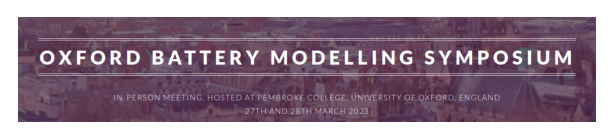
\includegraphics[width=0.85\textwidth]{./floats/logos/obms23.eps}
	% 	\end{center}
	% \end{minipage}
	% \hfill
	% \begin{minipage}{0.2\textwidth}
	% 	\begin{center}
	% 		
\includegraphics[width=0.85\textwidth]{./floats/logos/acomrwth.eps}
	% 	\end{center}
	% \end{minipage}
	% \hfill
	% \begin{minipage}{0.2\textwidth}
	% 	\begin{center}
	% 		
\includegraphics[width=0.5\textwidth]{./floats/logos/fzj.eps}
	% 	\end{center}
	% \end{minipage}
	%
	% \vspace{-0.6em}
	% \begin{minipage}{0.3\textwidth}
	% 	\begin{center}
	% 		
\includegraphics[width=0.45\textwidth]{./floats/logos/oxford_blue_obms23.eps}
	% 	\end{center}
	% \end{minipage}
	% \hfill
	% \begin{minipage}{0.3\textwidth}
	% 	\begin{center}
	% 		
\includegraphics[width=0.35\textwidth]{./floats/logos/acomrwth.eps}
	% 	\end{center}
	% \end{minipage}
	% \hfill
	% \begin{minipage}{0.3\textwidth}
	% 	\begin{center}
	% 		
\includegraphics[width=0.25\textwidth]{./floats/logos/fzj.eps}
	% 	\end{center}
	% \end{minipage}
	% \vspace{-0.6em}
	%
	% \vspace{-0.05em}
	\vspace{-1mm}
	\begin{minipage}{0.1\textwidth}
		\begin{flushright}
			
\includegraphics[width=1.1\textwidth]{./floats/logos/bosch_spring_school_2024Mar.eps}
		\end{flushright}
	\end{minipage}
	\hfill
	\begin{minipage}{0.3\textwidth}
		\begin{flushleft}
			\includegraphics[width=0.75\textwidth]{./floats/logos/bss24.eps}
		\end{flushleft}
	\end{minipage}
	% \hfill
	% \begin{minipage}{0.05\textwidth}
	% 	% \begin{center}
	% 	\psfrag{obms}[c][c] {$\hphantom{aaaaaaaaaa}\textbf{\#OBMS2023}\hphantom{aaaaaaaaaa}$}
	% 	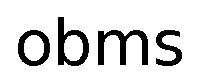
\includegraphics[width=0.85\textwidth]{./floats/logos/obms23_hashtag.eps}
	% 	% \end{center}
	% \end{minipage}
	\hfill
	\begin{minipage}{0.2\textwidth}
		\begin{flushright}
			
\includegraphics[width=0.9\textwidth]{./floats/logos/acomrwth.eps}
		\end{flushright}
	\end{minipage}
	\hfill
	\begin{minipage}{0.2\textwidth}
		\begin{flushleft}
			
\includegraphics[width=0.5\textwidth]{./floats/logos/fzj.eps}
		\end{flushleft}
	\end{minipage}
	\vspace{-5mm}
}
\end{document}
% ----------------------------------------------------------------------------------------------------------------